\documentclass[a4paper,12pt]{article}
\usepackage{amsmath, amssymb, graphicx}
\graphicspath{ {D:/Education/ATMOCN_630/hw3/} }

\DeclareMathAlphabet{\mathcal}{OMS}{cmsy}{m}{n}
\SetMathAlphabet{\mathcal}{bold}{OMS}{cmsy}{b}{n}
\newcommand{\bigO}{\mathcal{O}}


\begin{document}

\title{\vspace{-4.0cm}Geostrophic Approximation}
\author{Ian Beckley
\\University of Wisconsin-Madison}

\date{12 Jan. 2021}

\maketitle

\subsection*{Horizontal Momentum Equations}
Recall that $-\delta p = g\rho\delta z$ (hydrostatic balance). The horizontal equations of motion (see "Navier-Stokes on a Rotating Sphere") can be rewritten in terms of geopotential ($\Phi = gz$).

\begin{align}
\frac{\vec{V_h}}{dt} = -f\vec{k} \times \vec{V} - \nabla_p \Phi + \vec{F}
\end{align}

The expanded coriolis term is

\begin{align}
-2\Omega \times \vec{V} = -2\pi\begin{vmatrix} \hat{i} & \hat{j} & \hat{k} \\ 0 & 0 & -f \\  u & v & w \end{vmatrix}\\
-fv \hat{i} + fu \hat{j}
\end{align}

such that horizontal equations of motion can be written

\begin{align}
\frac{du}{dt} = -fv - \frac{\partial \Phi}{\partial x} + F_x\\
\frac{dv}{dt} = fu + \frac{\partial \Phi}{\partial y} + F_y
\end{align}

\subsection*{Geostrophic Wind}
Forgoing the friction term is acceptable aloft of the boundary layer, and we can again form geostrophic balance and define the geostrophic winds.

\begin{align}
\frac{du}{dt} = 0 = -fv - \frac{\partial \Phi}{\partial x}\\
fv = -\frac{d\phi}{dx}\\
\boxed{v_g = -\frac{1}{f}\frac{\partial \Phi}{\partial x}}
\end{align}

\begin{align}
\frac{dv}{dt} = 0 = fu - \frac{\partial\Phi}{\partial y}\\
fu = \frac{d\Phi}{dy}\\
\boxed{u_g = \frac{1}{f}\frac{\partial \Phi}{\partial y}}
\end{align}

Recall that these can also be evaluated with the pressure gradient via substitution of hydrostatic balance ($\delta p = -\rho g\delta z$). This may be easier for a surface pressure map, while aloft the height coordinate version will be more useful. 

\subsection*{Non-Divergence Theorem}
Another rendition of the non-divergence theorem is shown within the "Navier-Stokes on a Rotating Sphere" notes using the geostrophic streamfunction. The process here is similar.

\begin{align}
\nabla \cdot \vec{V_g} = \frac{\partial u_g}{\partial x} + \frac{\partial v_g}{\partial y}
\end{align}

Substituting (8) and (11),

\begin{align}
-\frac{1}{f}\frac{\partial}{\partial x}\frac{\partial \Phi}{\partial y} + \frac{1}{f}\frac{\partial}{\partial y}\frac{\partial \Phi}{\partial x} = 0
\end{align}

Thus, the geostrophic wind is non-divergent. Without convergence and divergence, however, there could be no vertical motion field. It follows that some portion of the total wind must be ageostrophic and responsible for divergence and convergence on our planet.

\subsection*{Geostrophic Paradox}
Another way to demonstrate the necessity of an ageostrophic wind component is by exploring the so called geostrophic paradox which is commonly illustrated using a zonal jet entrance region.

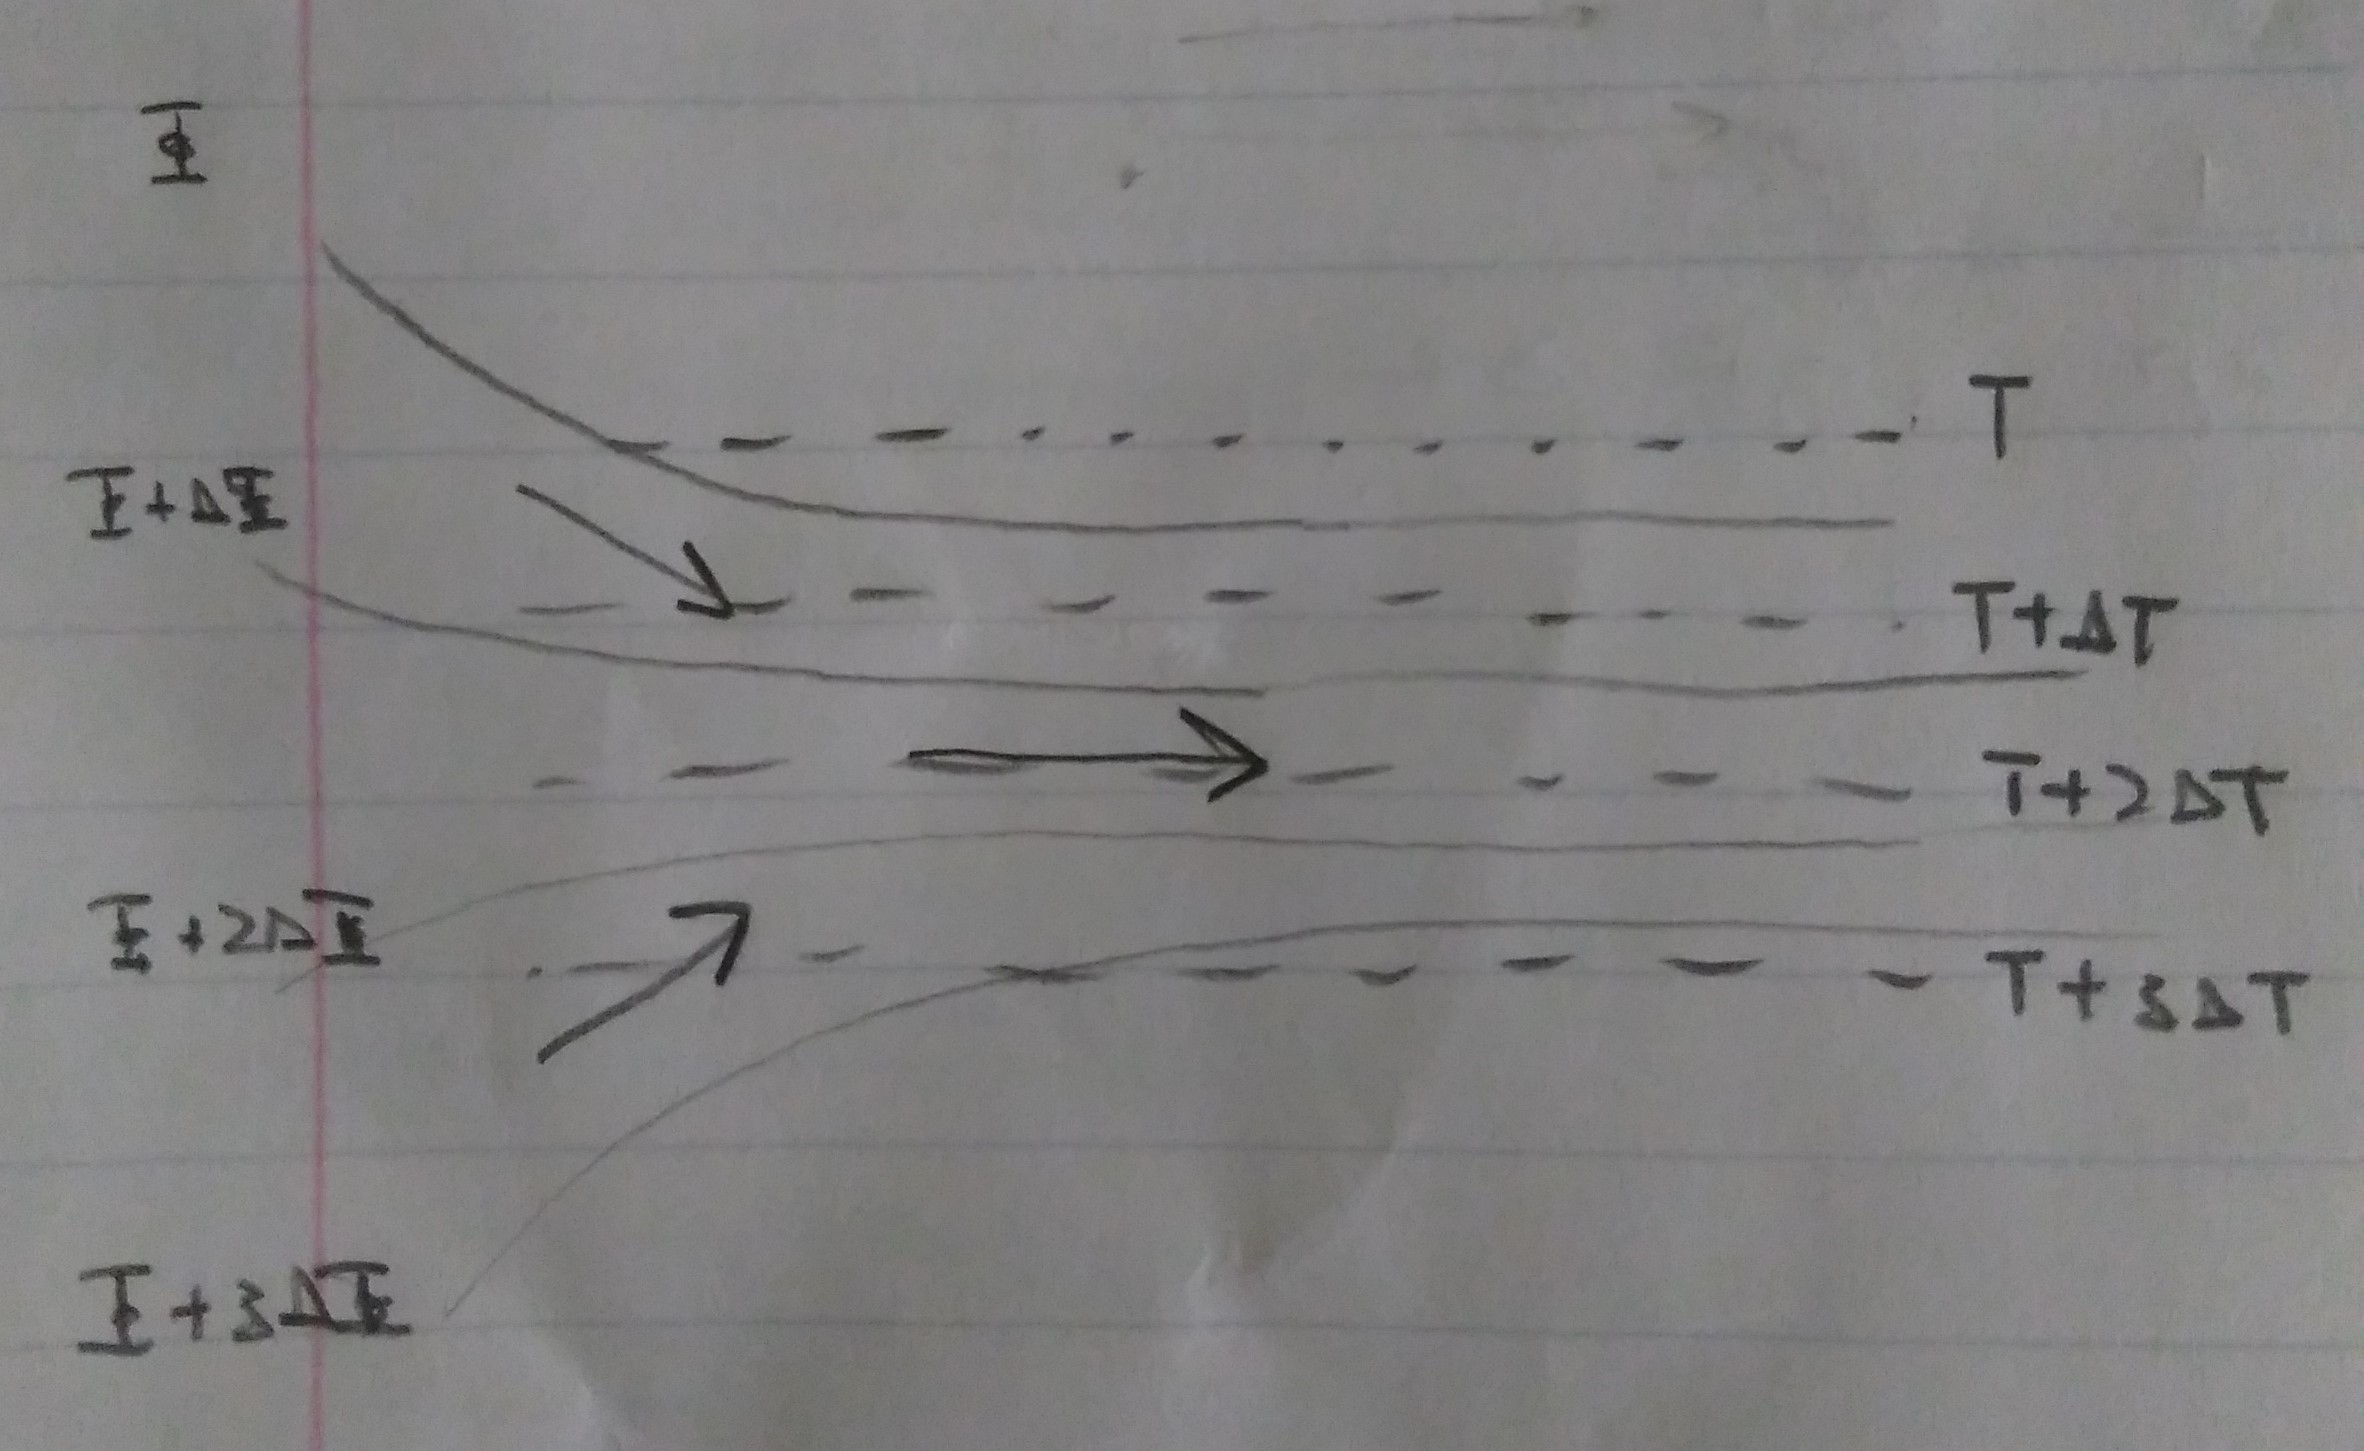
\includegraphics[width = \textwidth]{geostrophic_approximation_1}

The dotted lines are isotherms, while solid lines are geopotentials. Arrows represent the geostrophic wind in that location. The zonal thermal wind balance can be simplified as $\frac{\partial u_g}{\partial z} \propto c\,\frac{\partial T}{\partial y}$. It follows that within the confluent flow the geostrophic wind is blowing accross isotherms producing frontogenesis (the temperature gradient is increasing). In order to retain thermal wind balance, an increase in the horizontal temperature gradient must be met with an increase in the vertical shear. Given our discussion of the interplay between temperature gradients, thickness gradients, and geopotential height, this portion of the paradox is perhaps intuitive. 

At the same time, however, the very same geostrophic flow advects low momentum air into the entrance region. This serves to reduce the local vertical shear and flies in the face of what we just evaluated from confluence. We know from our discussion of the thermal wind that it cannot be responsible for temperature advections, so how can we expect the horizontal temperature gradient to relax, thereby retaining thermal wind balance. Clearly there must be some secondary ageostrophic circulation which serves to decrease the strength of the horizontal temperature gradient. Armed with the non-divergence theorem, one might accurately assume that vertical motion is the mechanism with which the temperature gradient is relaxed.


\subsection*{Rossby Number}
We can use the Rossby number to evaluate the validity of the geostrophic approximation. The Rossby number is defined as the ratio of the horizontal acceleration and coriolis force and alternatively as the ratio between the flow speed and product of the coreolis parameter and length scales.

\begin{align}
\boxed{R_0 = \frac{|\frac{du}{dt}|}{fv} \sim \frac{U}{fL}}
\end{align}

On the synoptic scale $f \sim 10^-4$, $L \sim 10^6$ and $U \sim 10$ such that $R_0 << 1$. Under this criteria $\vec{V}$ is well approximated as $\vec{V_g}$. If $R \sim 1$ it should be clear that the pressure gradient force is dominating the coriolis force, and the geostrophic approximation should not be made.
\end{document}